First, we analyze the size of the tested NFA constructions on the sample of practical regular expressions. There were four resulting NFAs constructed: Thompson, Glushkov, follow, and the partial derivative NFA. The position construction creates an identical NFA to Glushkov, and the partial derivative NFA has been constructed using nfaPDO, nfaPDRPN, and nfaPDDAG methods. Secondly, we analyze the performance of each membership evaluation algorithm independently on practical and randomly generated regular expressions. Membership is tested on each of the seven NFA constructions using the standard NFA membership algorithm that tracks a set of current states as each symbol of the input word is consumed. Additionally, three non-NFA methods were tested: backtracking, partial derivatives (pd), and optimized partial derivatives (pdo). Table \ref{tbl:Summary of algorithms} shows a summary of the tested methods below. The pdo algorithm was created too late into this thesis to test on randomly generated regular expressions, and the backtracking algorithm frequently experienced exponential membership time for the random sample, so neither of these methods were completed for the randomly generated sample.

\begin{table}[H]
  \doublespacing
  \centering
  \begin{tabular}{l| |c c l}
                & \multicolumn{2}{c}{Expression Type} \\
    Algorithm   & Practical & Random & Description \\
    \hline
    \hline
    Thompson    & Yes & Yes & Thompson construction \\
    Glushkov    & Yes & Yes & Glushkov construction \\
    Position    & Yes & Yes & Position construction \\
    Follow      & Yes & Yes & $\epsilon$-free follow construction \\
    PDO         & Yes & Yes & Optimized partial derivative construction \\
    PDRPN       & Yes & Yes & Partial derivative construction with string keys \\
    PDDAG       & Yes & Yes & Partial derivative construction using a DAG \\
    \hline
    pd          & Yes & Yes & Partial derivatives (non-NFA) \\
    pdo         & Yes & No  & Partial derivatives (non-NFA) with string keys \\
    backtrack   & Yes & No  & Exponential backtracking
  \end{tabular}
  \caption{Summary of tested algorithms}
  \label{tbl:Summary of algorithms}
\end{table}


\section{NFA Sizes for Practical Regular Expressions}
\label{sec:NFA Sizes for Practical Regular Expressions}
An indication of an NFA's efficiency is its size. So, given practically sampled regular expressions, how large are the resulting NFAs by their regular expression tree length? We have $12,023$ unique practical regular expressions, each with two forms: partial matching and non-partial matching. Since partial matching regular expression $\alpha$ might be equivalent to non-partial matching regular expression $\beta$ ($\alpha \neq \beta$), only one of $\alpha, \beta$ is kept. After considering this, we have $23,253$ unique regular expressions. If any construction takes longer than two minutes, it is preempted and thrown away. Table \ref{tbl:nfa sizes} shows that the PDO method is the most limiting factor for these constructions, and as such we have $23,247$ regular expressions that are successful for all construction methods. This table also shows the amount of time it took to construct the regular expressions into NFAs, but this measurement should be taken \emph{very lightly} since the number of regular expressions for each method may be unequal, and that it was performed on a personal computer instead of a server.

\begin{table}[H]
  \center
  \begin{tabular}{l|c|c}
    Method & \# Regular Expressions & Time taken (s) \\
    \hline
    Follow     & 23,253 & 26.968 \\
    Glushkov   & 23,253 & 36.084 \\
    Position   & 23,253 & 38.332 \\
    PDDAG      & 23,253 & 73.251 \\
    Thompson   & 23,251 & 141.28 \\
    PDRPN      & 23,251 & 260.19 \\
    PDO        & 23,247 & 680.46 \\
  \end{tabular}
  \caption{The number of regular expressions constructed by method without preemption}
  \label{tbl:nfa sizes}
\end{table}

Figure \ref{fig:nfa_sizes} plots the sizes of different NFAs for all $23,247$ non pre-empted regular expressions common to every construction method. We correctly assert that PDO, PDDAG, and PDRPN all construct the same partial derivative NFA; as well, the Glushkov and position constructions build an identical NFA. Partial derivative constructions create the smallest NFA, then the follow construction, position/Glushkov, and finally the Thompson NFA.

\begin{figure}[H]
  \center
  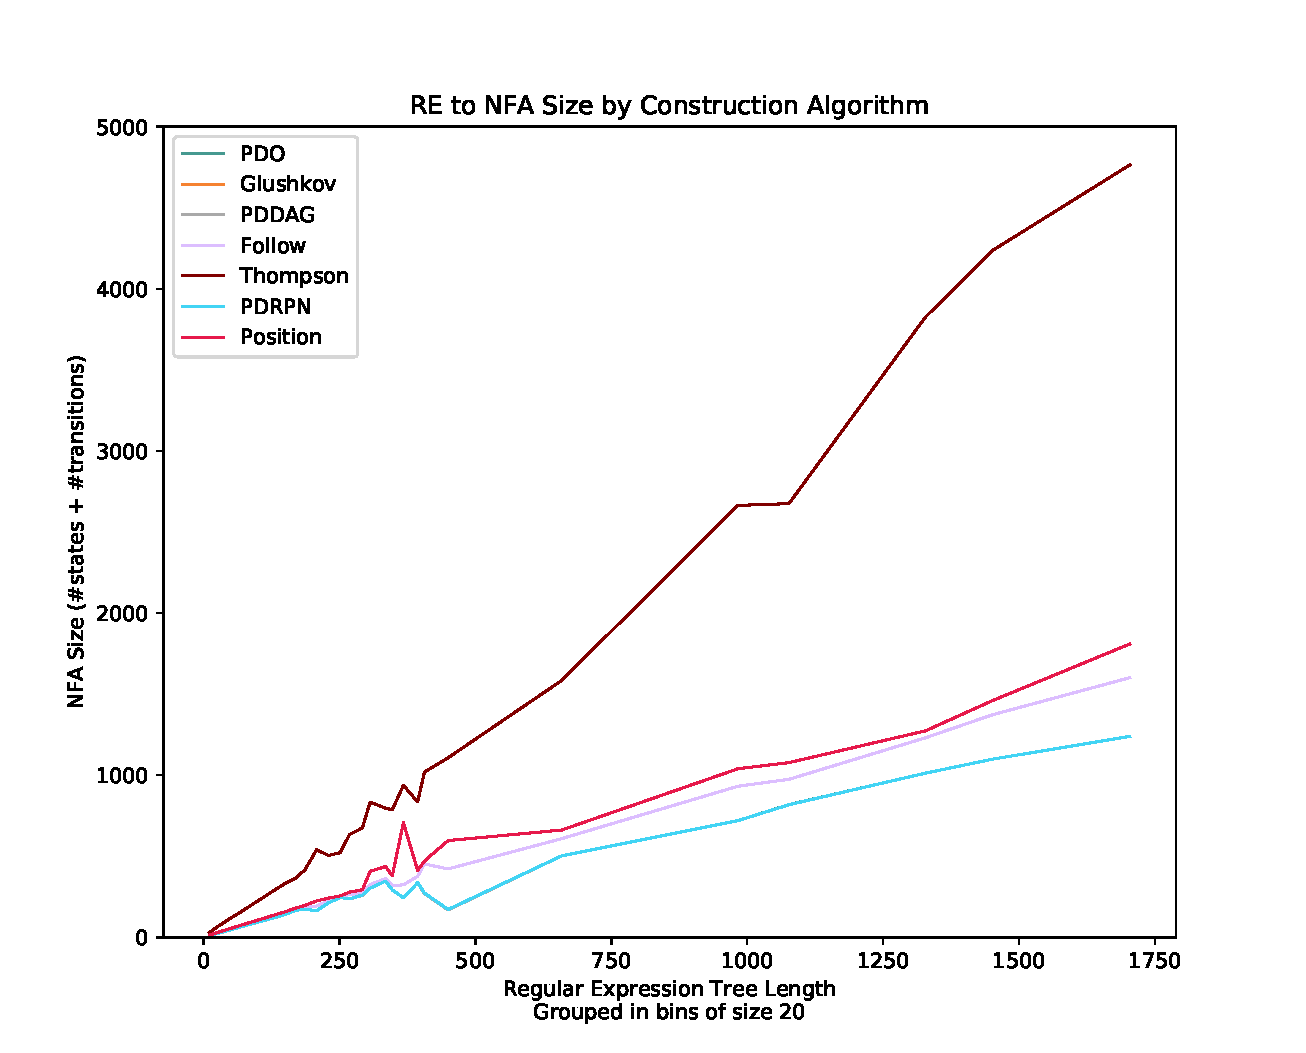
\includegraphics[width=0.75\linewidth]{fig/nfa_sizes}
  \caption{Sizes of the NFAs produced using different construction methods and practical regular expressions}
  \label{fig:nfa_sizes}
\end{figure}





\section{Practical Regular Expressions}
\label{sec:Practical Regular Expressions}
We found 12,023 unique regular expressions that could be successfully converted into their equivalent mathematical syntax. Due to time constraints, only 10,686 regular expressions have been fully tested using each method. Table \ref{tbl:practical sample by tree length} shows the distribution of the sampled practical regular expressions by their tree length, and the quantity that have been fully tested. Beyond tree length 175, we only have single-digit quantities and we are therefore not confident to make any conclusions; all plots of measuring the performance of practical regular expressions will only include regular expressions with tree length less than 180 (of which we have  $\approx$10,662, depending on the unimportant distribution within $[175, 200)$).

\begin{table}[H]
  \center
  \begin{tabular}{c|c|c}
    Tree Length & \# Expressions & \# Completed \\
    \hline
    $[0, 25)$     & 8,053 & 7,185 \\
    $[25, 50)$    & 2,560 & 2,305 \\
    $[50, 75)$    & 832   & 747 \\
    $[75, 100)$   & 272   & 239 \\
    $[100, 125)$  & 136   & 98 \\
    $[125, 150)$  & 79    & 55 \\
    $[150, 175)$  & 49    & 30 \\
    $[175, 200)$  & 10    & 3
    % Total:        11,991  10,662
  \end{tabular}
  \caption{The number of practical regular expressions by tree length}
  \label{tbl:practical sample by tree length}
\end{table}

\begin{figure}[H]
  \center
  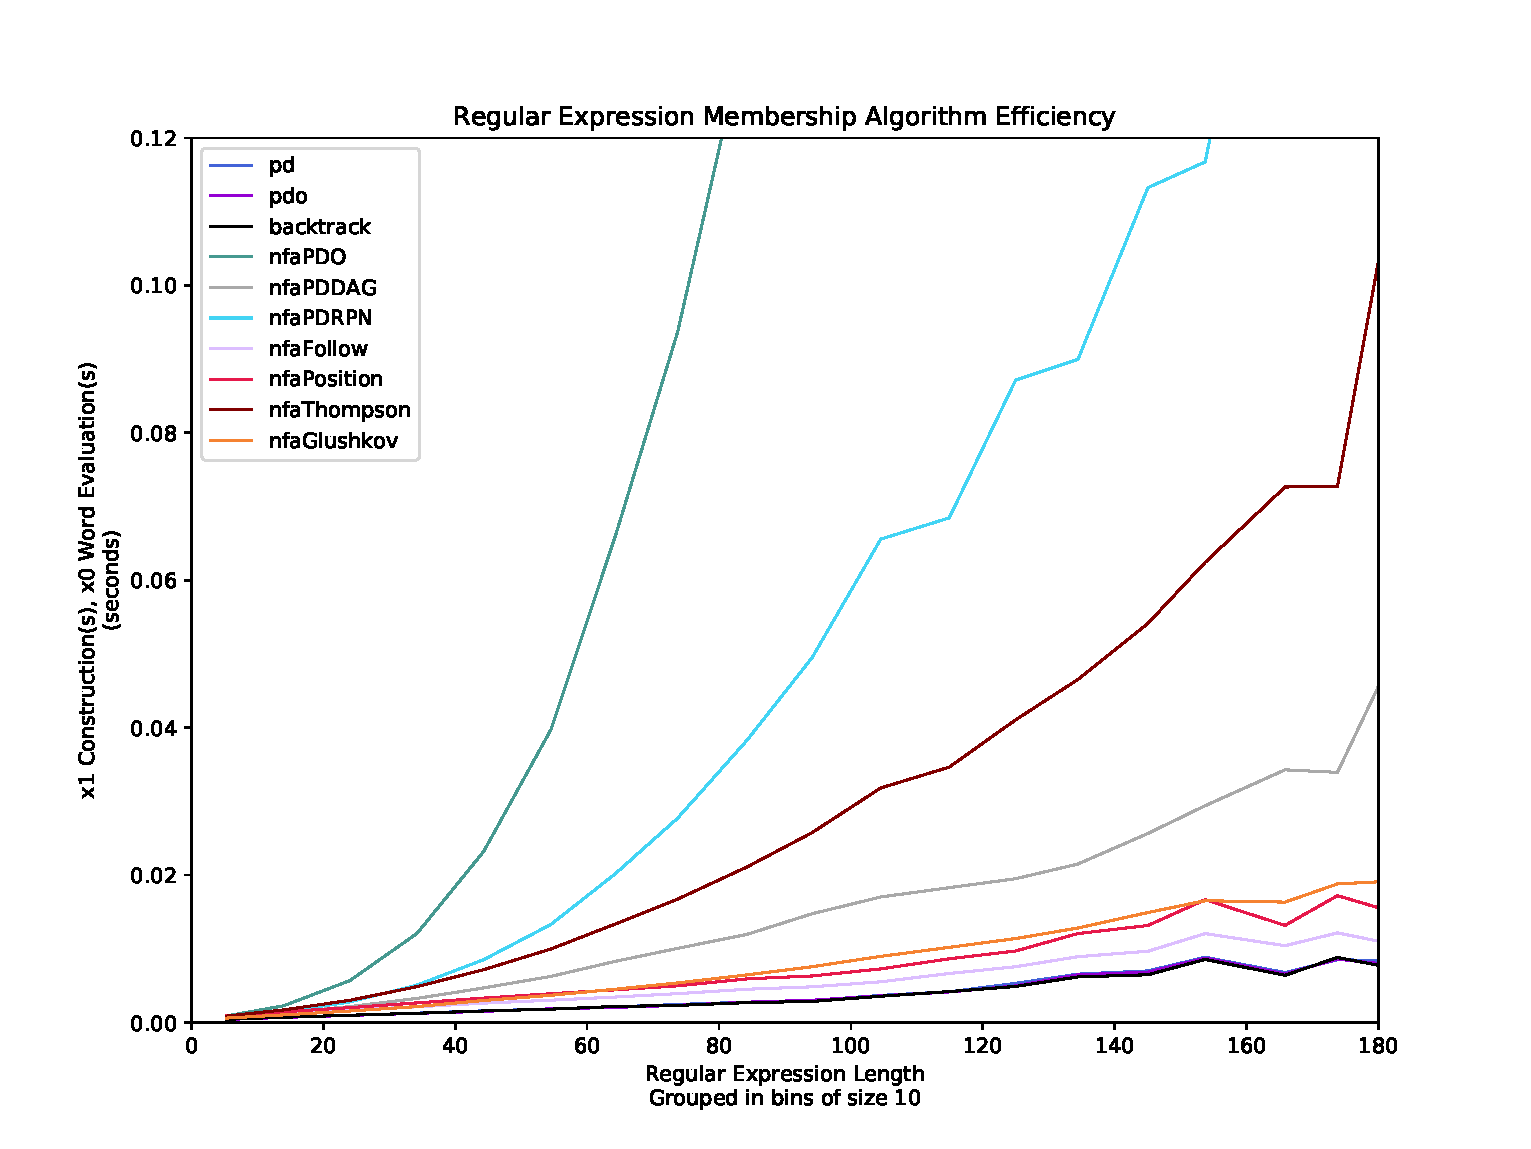
\includegraphics[width=0.75\linewidth]{fig/prac/1construction}
  \caption{Construction time by method for practical regular expressions}
  \label{fig:prac/1construction}
\end{figure}

Figure \ref{fig:prac/1construction} shows the time taken to construct an appropriate Python class object starting at a mathematical regular expression string. As expected, the methods which do not construct an NFA represent the fastest constructions (pd, pdo, and backtrack all have an identical construction into a partial matching regular expression tree). The remaining NFA constructing methods are given in increasing order: follow, position, Glushkov, nfaPDDAG, Thompson, nfaPDRPN, and finally nfaPDO.

Once the structure is constructed, we must consider the efficiency of the different membership algorithms. Figure \ref{fig:prac/1evaluation} compares the different methods. Both non-NFA partial derivative algorithms (pd and pdo) are significantly slower to evaluate word membership than all other tested methods. The backtracking algorithm is frequently the fastest, but occasionally experiences spikes where excessive backtracking was required. The NFAs are divided into two classes according to membership time: sequential NFAs (PDO/PDRPN/PDDAG, Glushkov/position, and follow), and the Thompson NFA with $\epsilon$-transitions. These empty transitions delay word matching and therefore result in a slower membership process. In reality, the backtracking algorithm occasionally failed all together when Python's maximum recursion depth (set to 12,000) was exceeded. Presumably, this issue could be solved by refactoring the backtracking algorithm to use an iterative approach, so any time the maximum recursion depth was reached, the regular expression was removed from our results set for every method.

\begin{figure}[H]
  \centering
  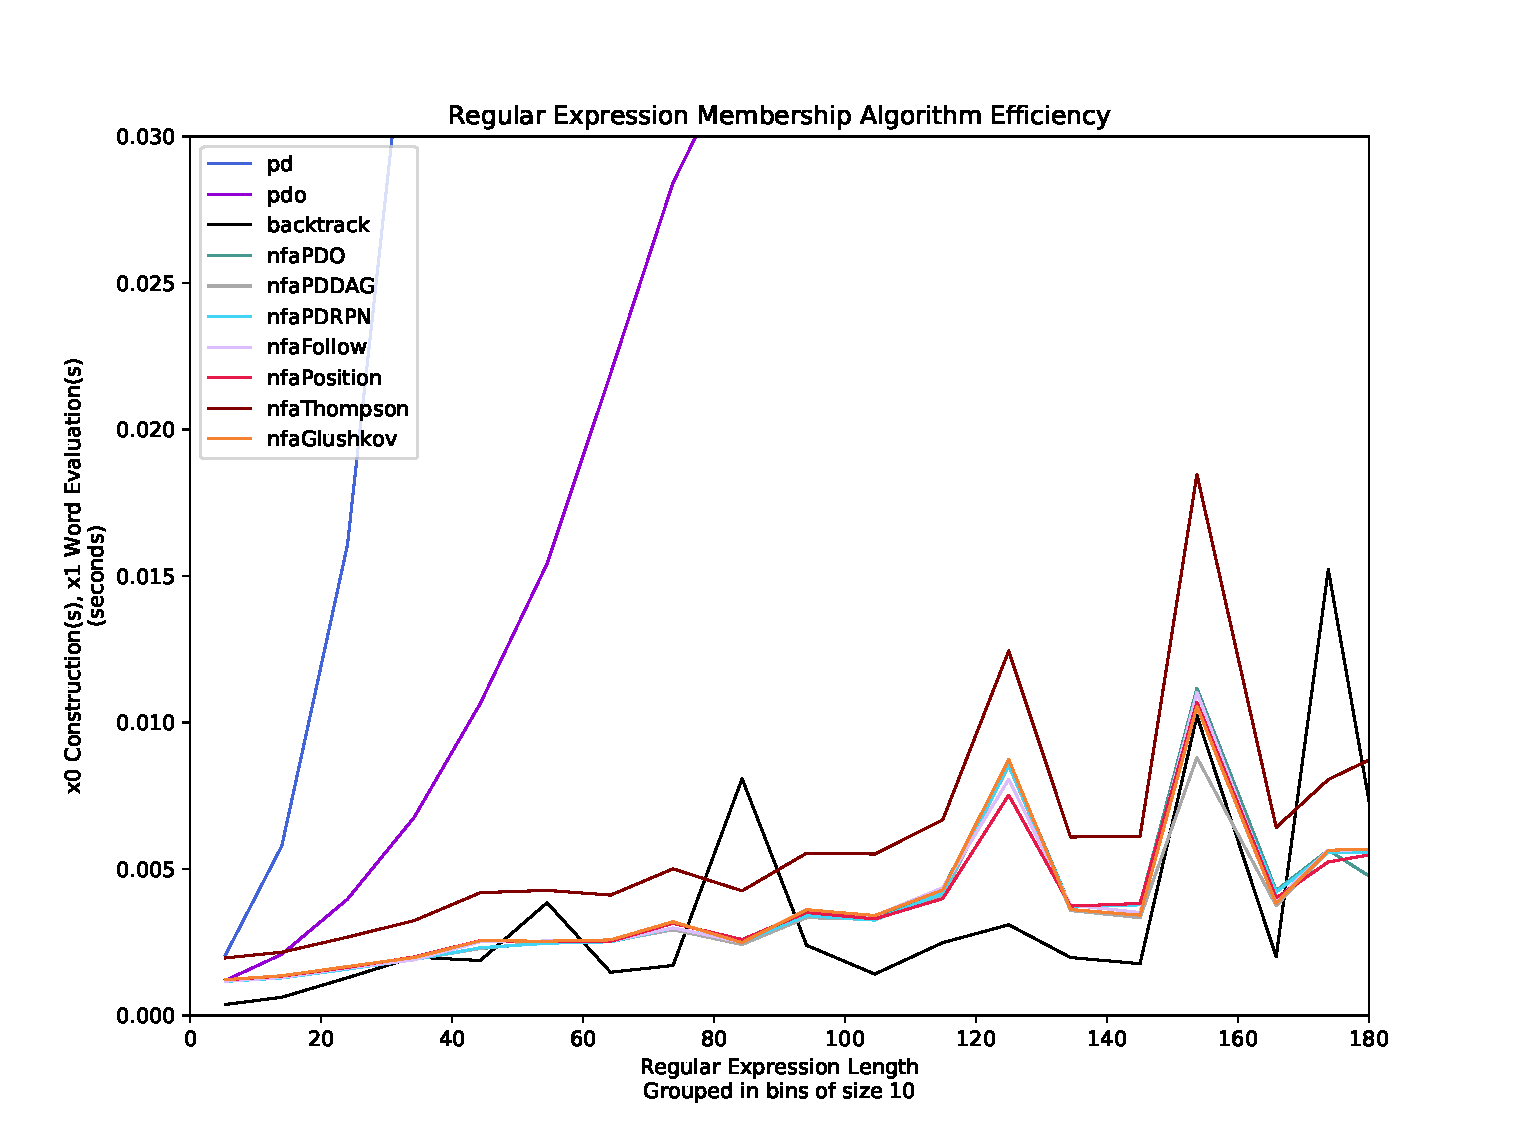
\includegraphics[width=0.75\linewidth]{fig/prac/1evaluation}
  \caption{Word membership time of practical regular expressions after construction has taken place}
  \label{fig:prac/1evaluation}
\end{figure}

Often, regular expressions are used to evaluate the membership of just a single input word. In this case, Figure \ref{fig:prac/1const1eval} compares solutions to the one-word membership problem using each of our algorithms. The backtracking algorithm continues to be impressively fast, due to its low construction cost and average fast membership time. The follow algorithm has a small edge over nearly equivalent position and Glushkov constructions. Then, with larger time gaps: nfaPDDAG, Thompson, pdo, nfaPDRPN, nfaPDO, and finally pd. This is very similar to Figure \ref{fig:prac/1construction} since word membership takes far less time on average than construction time.

\begin{figure}[H]
  \center
  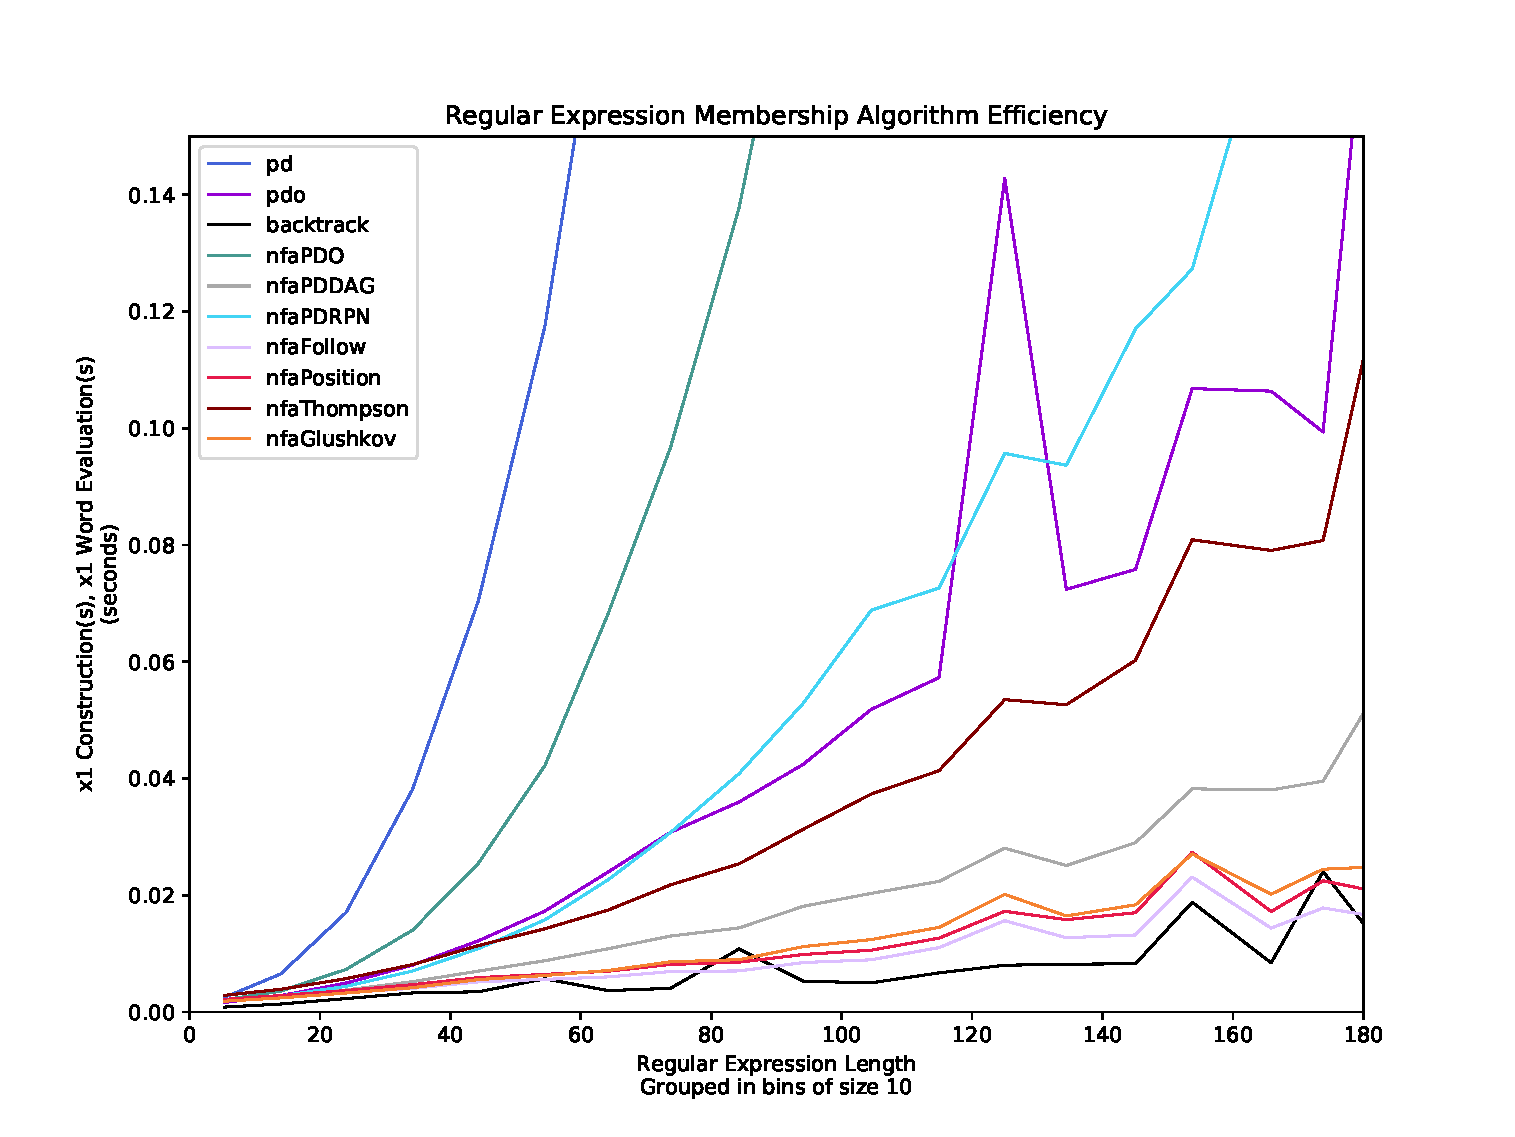
\includegraphics[width=0.75\linewidth]{fig/prac/1const1eval}
  \caption{Sum of construction time and one-word membership time for practical regular expressions}
  \label{fig:prac/1const1eval}
\end{figure}

A key observation from Figure \ref{fig:prac/1const1eval} is the pdo algorithm is faster on average than the nfaPDO and nfaPDRPN methods. The partial derivative NFA is constructed by considering \emph{every} possible partial derivative with respect to \emph{every} alphabet symbol, but the (non-NFA) partial derivative algorithm only computes the partial derivatives with respect to the specific input word. Equivalently, only a subset of the states in the partial derivative NFA are useful for the computation for a given input word; so the overall computation cost can be mitigated by only constructing the useful states. The pdo algorithm is based on the same methodology as the nfaPDRPN construction, and it makes sense that pdo is faster when considering a single input word. Using nfaPDDAG as inspiration, there should be a (non-NFA) partial derivative algorithm which computes membership faster than PDDAG can be constructed and membership evaluated; but to our knowledge no such algorithm currently exists.

Perhaps the regular expression is used to filter data from a database with 100,000 records. Figure \ref{fig:prac/1const10e6eval}(a) shows that as long as the regular expression library is using a sequential NFA to decide membership, there is little relative difference between construction algorithms. With so many word evaluations, even the slow nfaPDO construction is acceptable. Because the overall time is dominated by word membership tests, the construction time is unimportant. NFAs compute all possible paths through the regular expression at construction-time, whereas pd, pdo, and backtrack algorithms do this at membership-time. The pd and pdo algorithms are blown away, but backtracking remains generally competitive assuming the expression is not vulnerable to catastrophic backtracking. Like in Figure \ref{fig:prac/1evaluation}, the sequential NFAs provide an advantage over the Thompson NFA. It is difficult to declare a clear winner among the sequential NFA methods, but Figure \ref{fig:prac/1const10e6eval}(b) attempts to do so by decreasing the resolution (using more averaging) and zooming into a focused region. The nfaPDDAG algorithm is the fastest, followed by the other partial derivative NFAs, and then nearly equivalent Glushkov, position, and follow NFA methods. 

\begin{figure}[H]
  \centering
  \begin{subfigure}[b]{0.45\linewidth}
    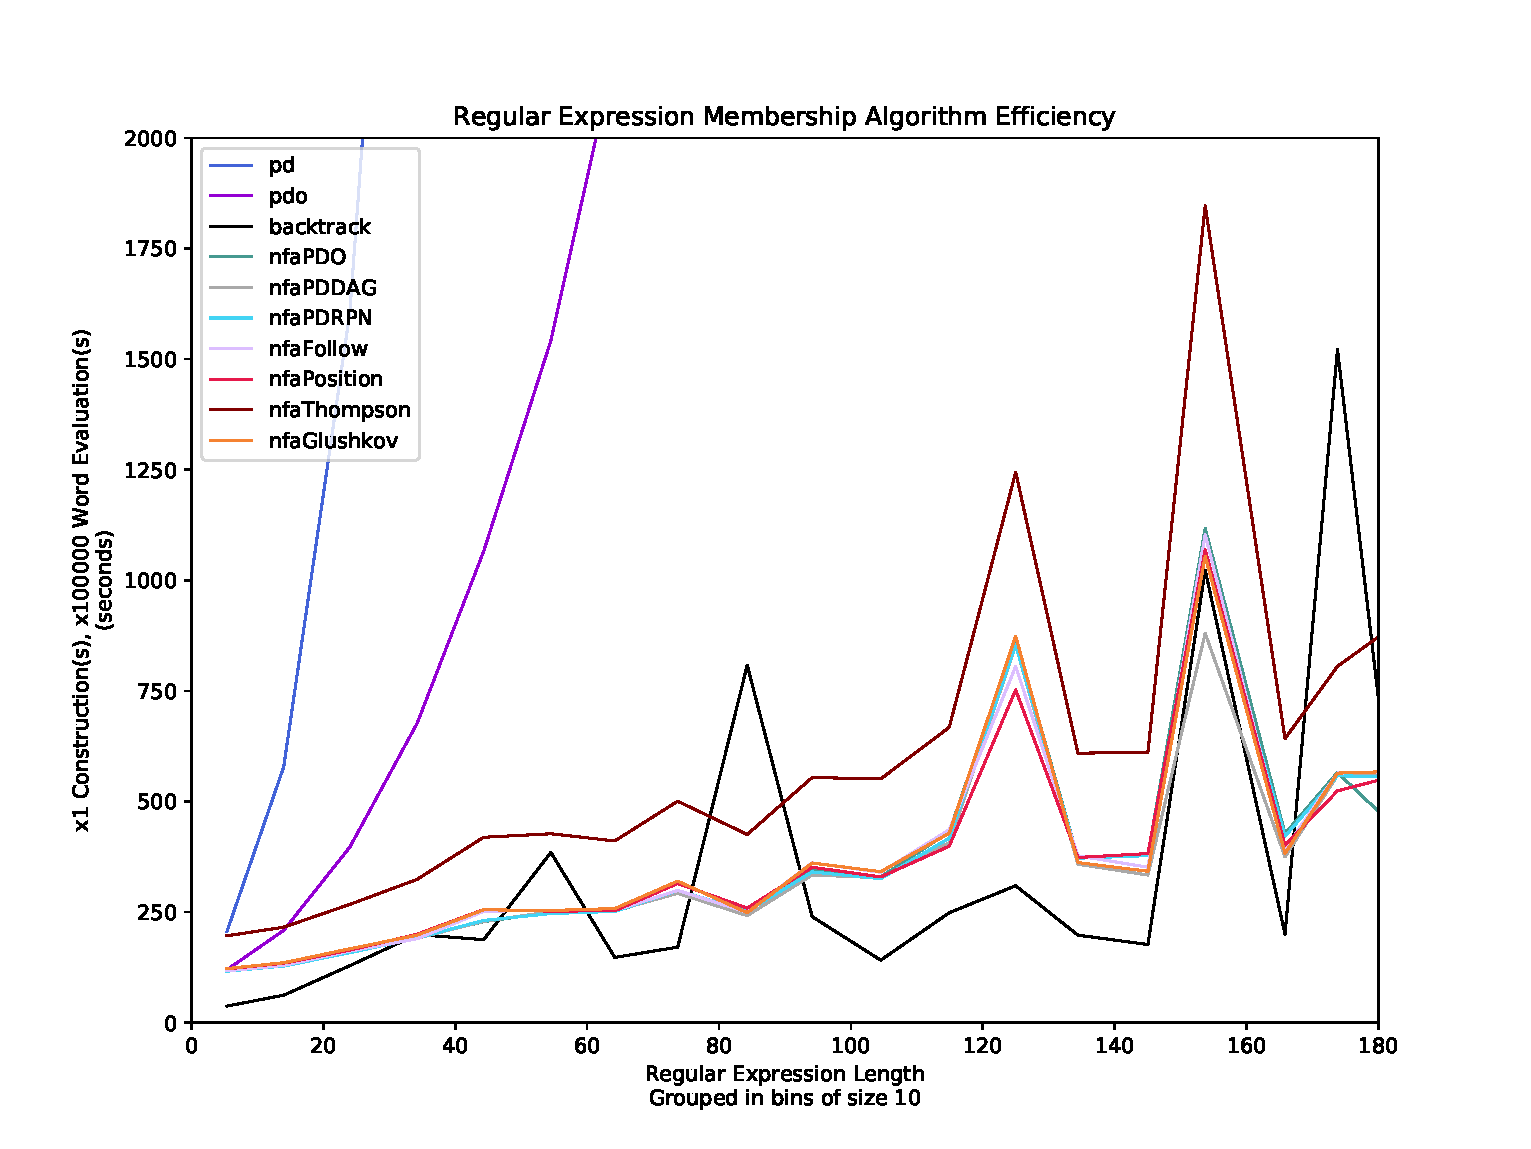
\includegraphics[width=\linewidth]{fig/prac/1const10e6eval}
    \caption{Full picture: length bins of tree length 10}
  \end{subfigure}
  \begin{subfigure}[b]{0.45\linewidth}
    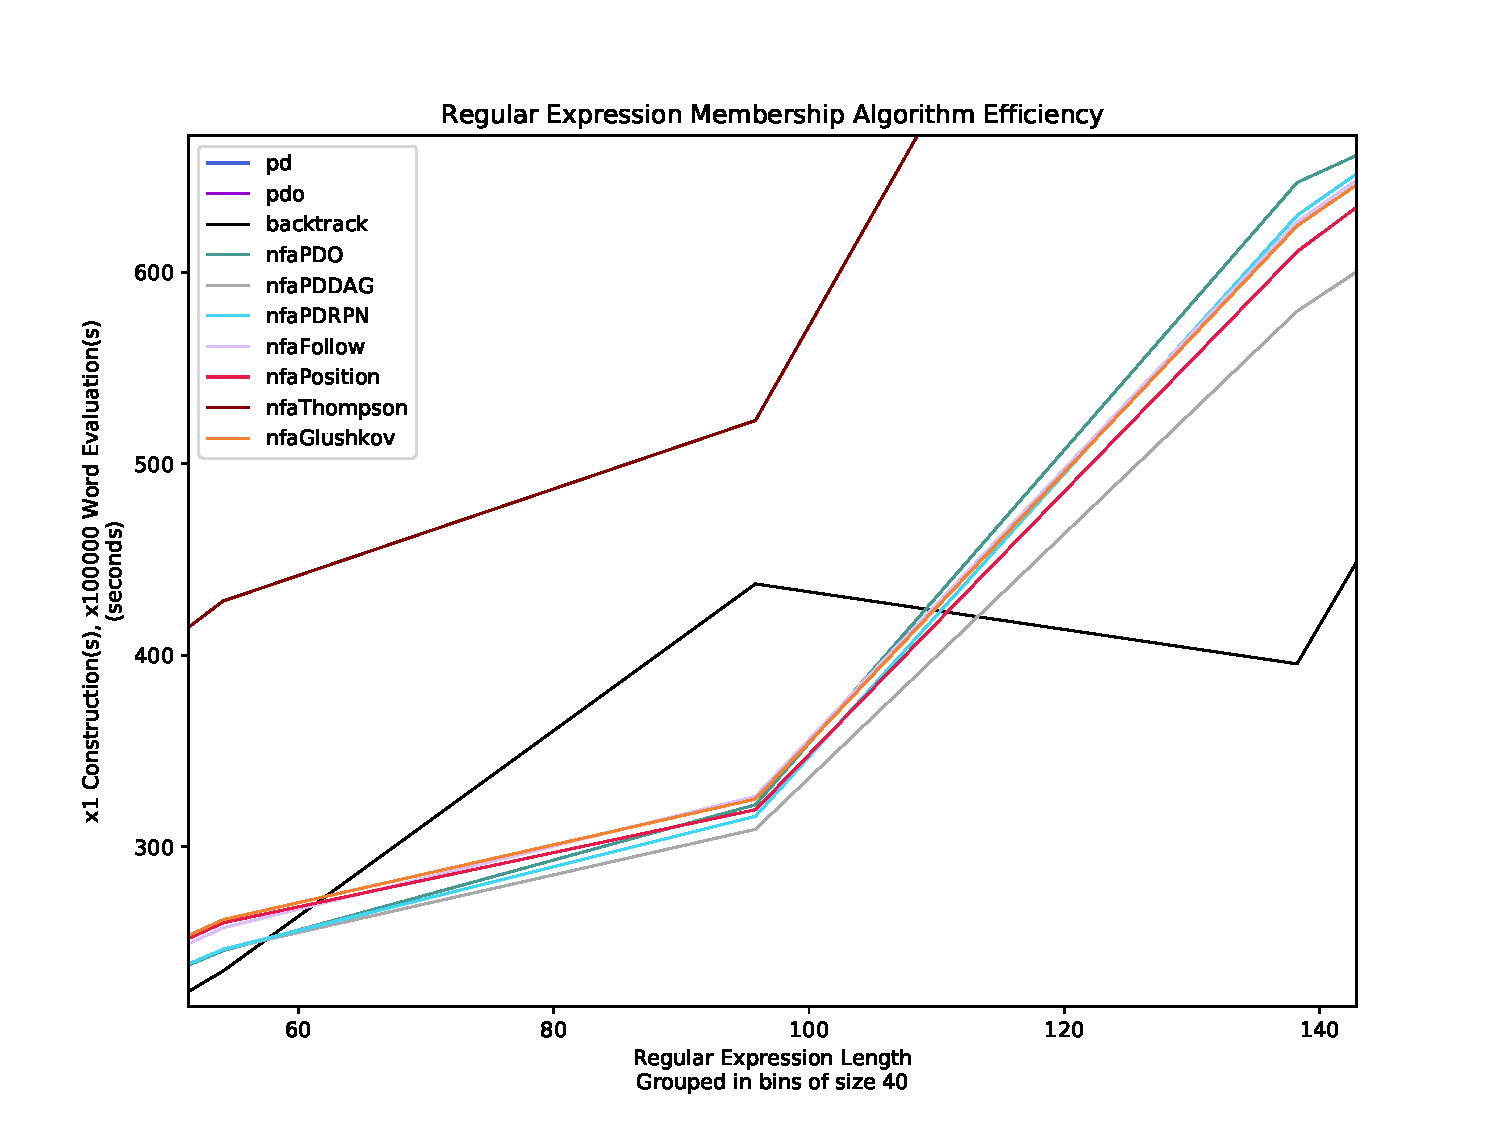
\includegraphics[width=\linewidth]{fig/prac/1const10e6eval_zoomed}
    \caption{Zoomed in: length bins of tree length 40}
  \end{subfigure}
  
  \caption{Sum of construction time and 100,000 word membership time for practical regular expressions}
  \label{fig:prac/1const10e6eval}
\end{figure}





\section{Randomly Sampled Regular Expressions}
\label{sec:Randomly Sampled Regular Expressions}
Using the same testing framework for randomly generated regular expressions allows us to compare the results with practical expressions. It also gives us more control and confidence: 784 regular expressions with alphabet of size $10$ were generated for each tree length \{25, 50, 100, 150, 200, 300, 400, 500\}. We were unable to sample many practical regular expressions beyond tree length 200, so this will give a much better picture how these algorithms perform for longer expressions. Once the tests are complete, we have a 95\% confidence interval with a 3.5\% margin of error. However once again, the test set is incomplete due to both time constraints and memory issues related to deeply nested star operations and pairwise (Section \ref{subsec:Pairwise Word Generation}) language generation within the set of randomly generated regular expressions. Table \ref{tbl:random sample by tree length} shows the amount each tree length has been completed. Instead, we are 95\% confident that our results are statistically correct with a margin of error no more than 5\% for all tree lengths except 500.

\begin{table}[H]
  \center
  \begin{tabular}{c|c|c}
    Tree Length & \# Expressions & \# Completed \\
    \hline
    $25$    & 784 & 783 \\
    $50$    & 784 & 780 \\
    $100$   & 784 & 769 \\
    $150$   & 784 & 741 \\
    $200$   & 784 & 688 \\
    $300$   & 784 & 581 \\
    $400$   & 784 & 422 \\
    $500$   & 784 & 286
    % Total:  6,272 5,050
  \end{tabular}
  \caption{The number of randomly generated regular expressions by tree length}
  \label{tbl:random sample by tree length}
\end{table}

The backtracking membership algorithm frequently experienced exponential membership time for randomly generated regular expressions. There are a few reasons why this could make sense: (1) programmers may be aware of catastrophic membership and therefore write their regular expressions to not be vulnerable, (2) vulnerable regular expressions may not be useful for GitHub developers, or (3) a small alphabet with nested star operations allow input words to be matched in complex ways. Because the backtracking algorithm was taking too long, it was disabled so the rest of the tests could be run in our lifetimes. In addition, the results for the pdo algorithm were not completed for the randomly generated set of regular expressions because the pdo algorithm was created only recently.

\begin{figure}[H]
  \center
  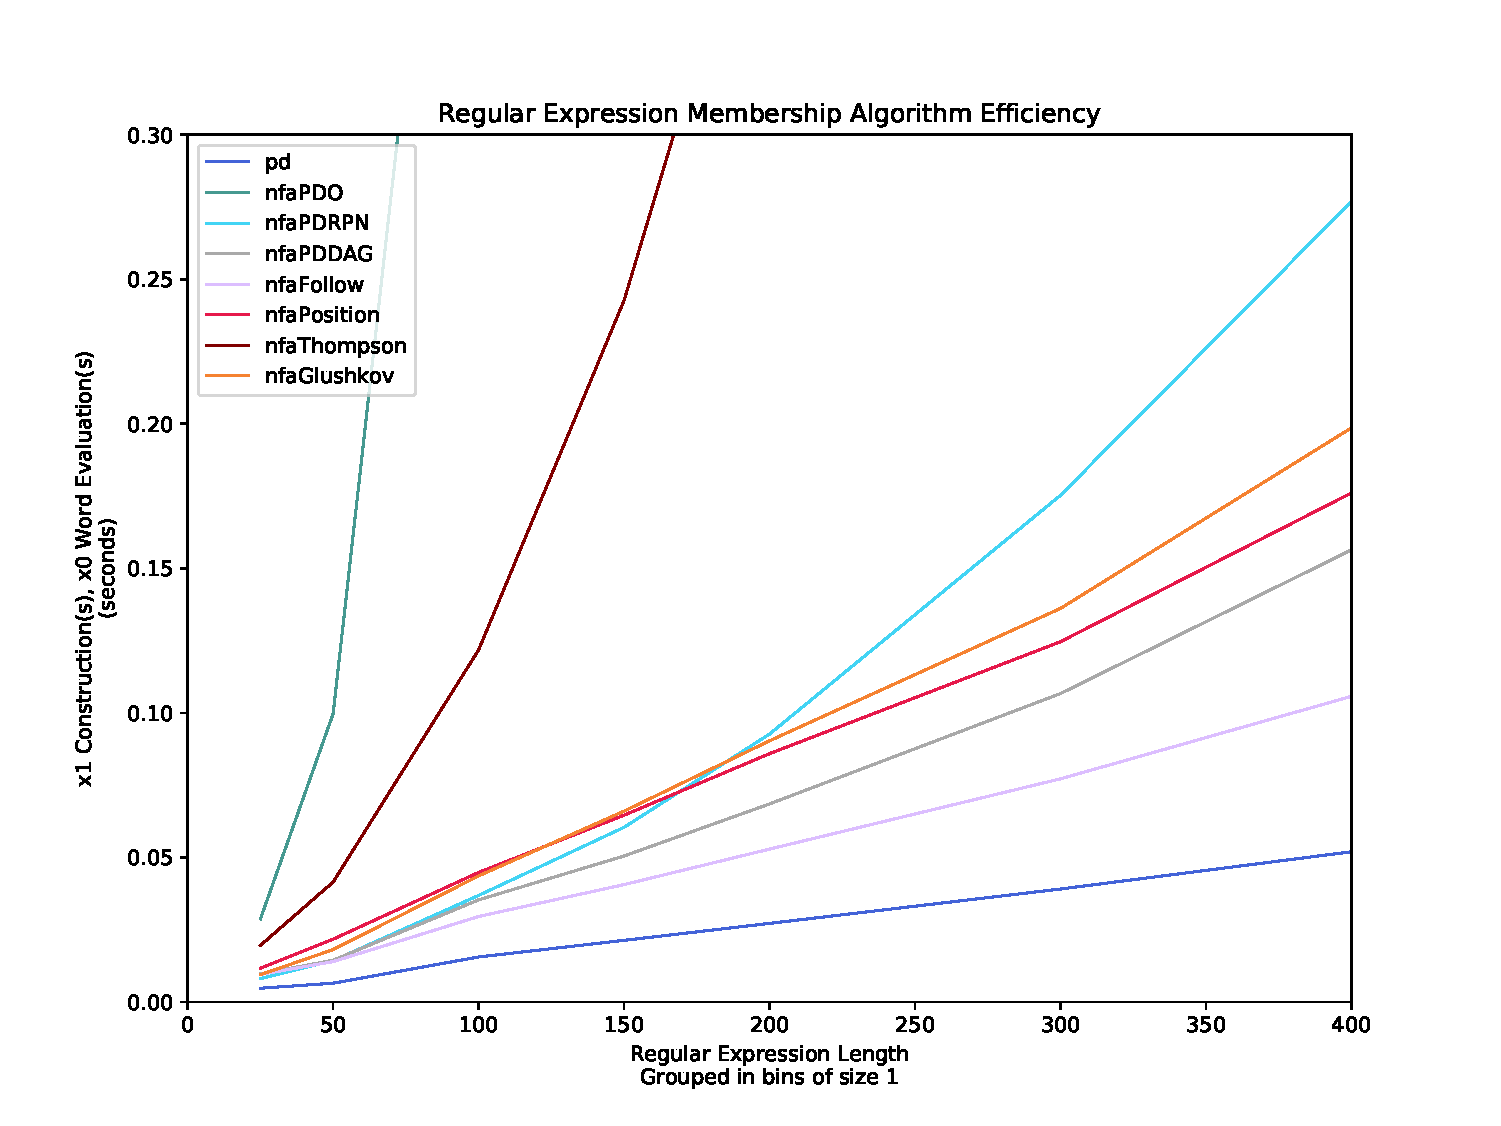
\includegraphics[width=0.75\linewidth]{fig/rand/1construction}
  \caption{Construction time by method for randomly generated regular expressions}
  \label{fig:rand/1construction}
\end{figure}

Figure \ref{fig:rand/1construction} shows the construction times for each of the algorithms. Once again the pd algorithm has the least construction time because it does not construct an NFA, and the nfaPDO and Thompson algorithms are very slow. All other sequential NFA constructions are given by increasing speed: follow, nfaPDDAG, position, Glushkov, and finally nfaPDRPN. It is exciting to see the nfaPDDAG algorithm performing so well; since the partial derivative NFA was previously so far out of reach with the nfaPDO method.

In Figure \ref{fig:rand/1evaluation} we get a look at word membership times. The time scale is significantly larger than with practical regular expressions because the accepted words are sometimes extremely long using the modified combination generation approach with deeply nested stars. However, the relative ranking of each method is still comparable because the exact same input words are generated for any given regular expression. The Thompson NFA continues to have $\epsilon$-transitions that delay word matching, and is therefore the slowest. Each of the partial derivative NFAs are very close (as they should be, since they generate the same NFA). The position algorithm appears to be slightly faster than follow, which is slightly faster than Glushkov. Remarkably for much of the domain, the (non-NFA) partial derivative algorithm is the fastest. And we would expect the pdo algorithm to speed up this computation even more. This is in direct contrast to practical regular expressions where the partial derivative algorithm is the slowest. Why are partial derivatives so much better in randomly generated regular expressions?

\begin{figure}[H]
  \center
  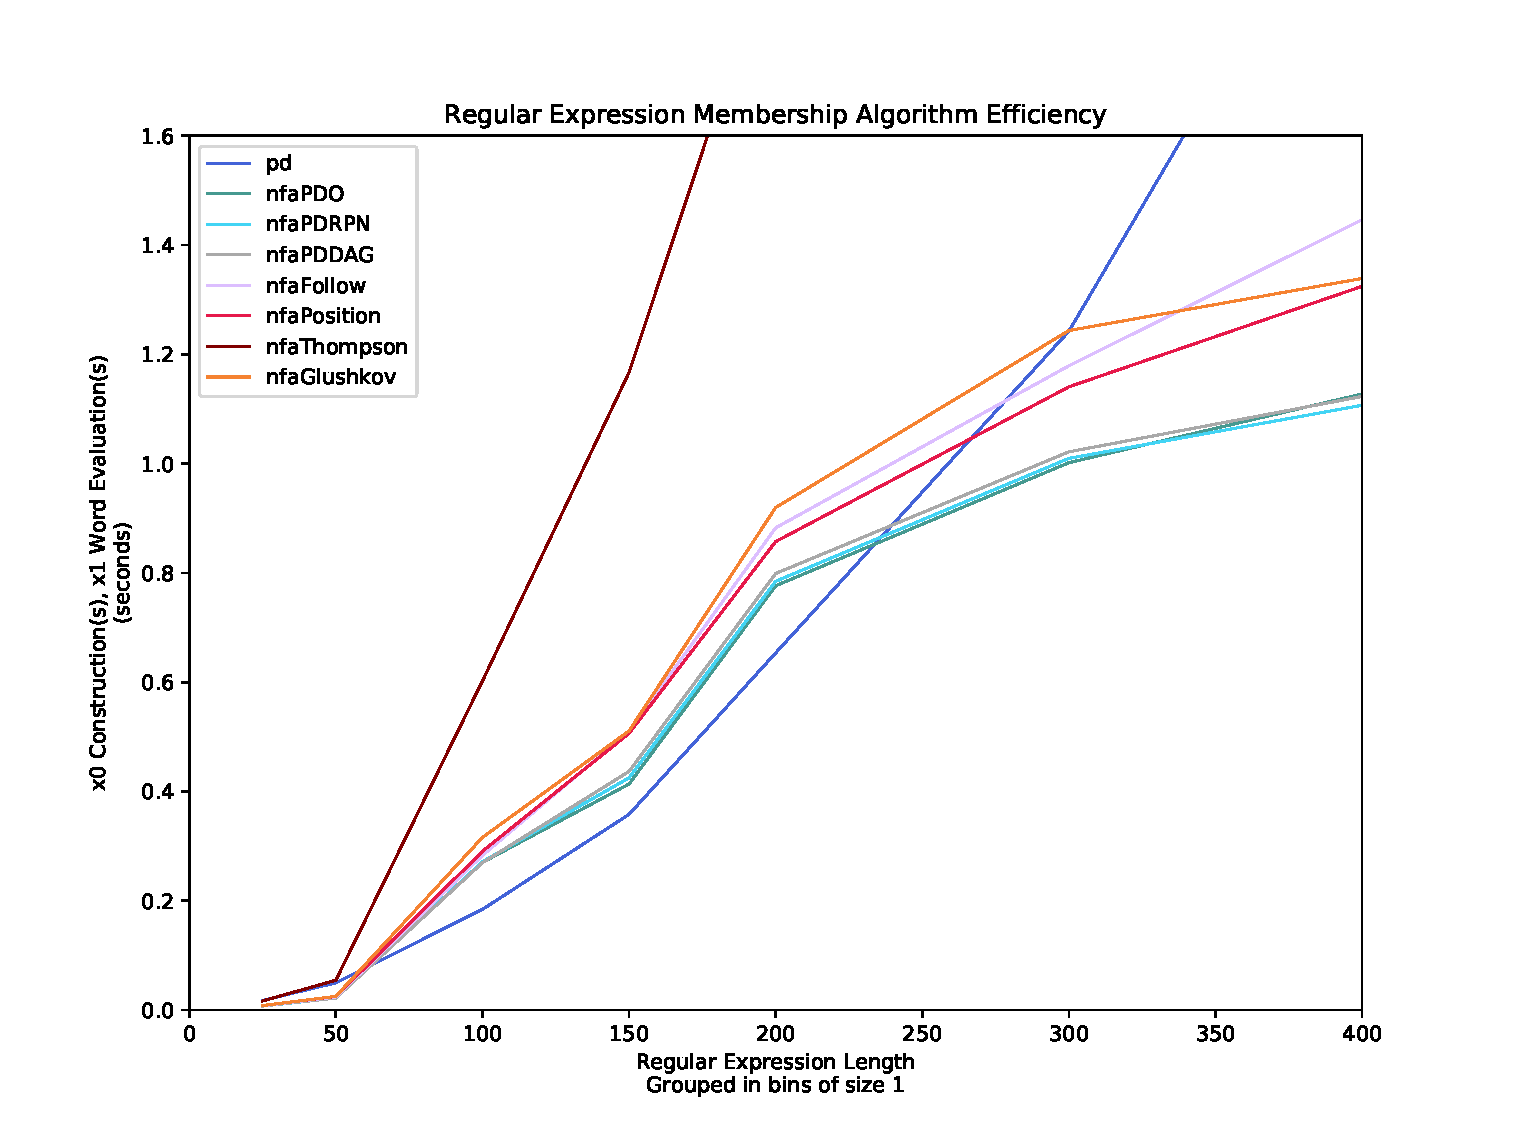
\includegraphics[width=0.75\linewidth]{fig/rand/1evaluation}
  \caption{Word membership time of randomly generated regular expressions after construction has taken place}
  \label{fig:rand/1evaluation}
\end{figure}

An analysis of the composition of practical and randomly generated regular expressions exposes a potential answer. Since membership is tested on regular expressions with partial matching enabled, this analysis first enabled partial matching on each expression before checking the relative frequency of internal nodes. Recall: optional operations are removed in favour for a disjunction with the empty word in the anchor elimination construction.

\begin{table}[H]
  \centering
  \begin{tabular}{r|c c}
    \empty & Practical Expressions & Random Expressions \\
    \hline
    Concatenation & $78.99\%$ & $43.02\%$ \\
    Disjunction   & $3.10\%$  & $41.93\%$ \\
    Star          & $17.91\%$ & $15.05\%$
  \end{tabular}
  \caption{Relative frequencies of internal nodes in the regular expression samples}
  \label{tbl:composition}
\end{table}

As shown in Table \ref{tbl:composition}, practically sampled regular expressions have almost twice as many concatenations as randomly generated expressions. Recall the partial derivative definition for concatenation from Section \ref{sec:Derivatives}:
\begin{center}
  $$
  \delta_\sigma(\alpha \beta) = \begin{cases}
    \delta_\sigma(\alpha)\{\beta\}                            & \epsilon \notin L(\alpha) \\
    \delta_\sigma(\alpha)\{\beta\} \cup \delta_\sigma(\beta)  & \epsilon \in L(\alpha)
  \end{cases}
  $$
\end{center}
Calculating the partial derivative set of a concatenation requires checking if the empty word is accepted by the left child ($\alpha$). Consider converting the programmer's regular expression $a\{6\}$ into the mathematical regular expression using methods from Section \ref{subsec:Converting into FAdo Compatible Syntax}. The tree in Figure \ref{fig:left vs right expansion}(a) is the result.
\begin{figure}[H]
  \centering
  \begin{subfigure}[b]{0.45\linewidth}
    \centering
    \Tree
    [
      .$\odot$
      [
        .$\odot$
        [
          .$\odot$
          [
            .$\odot$
            [
              .$\odot$
              a
              a
            ]
            a
          ]
          a
        ]
        a
      ]
      a
    ]
    \caption{Left expansion}
  \end{subfigure}
  \begin{subfigure}[b]{0.45\linewidth}
    \centering
    \Tree
    [
      .$\odot$
      a
      [
        .$\odot$
        a
        [
          .$\odot$
          a
          [
            .$\odot$
            a
            [
              .$\odot$
              a
              a
            ]
          ]
        ]
      ]
    ]
    \caption{Right expansion}
  \end{subfigure}
  \caption{Converting $a\{6\}$ into a mathematical regular expression}
  \label{fig:left vs right expansion}
\end{figure}
Observe how in Figure \ref{fig:left vs right expansion}(a) the left child represents a larger subtree than the right child. If this tree were evaluated for partial derivative membership on the word $a^6$, the left subtrees would need to be traversed repeatedly to check if it accepts the empty word. If the tree grew to the right like in Figure \ref{fig:left vs right expansion}(b), checking if the left subtree accepts the empty word is a much faster operation.

\begin{figure}[H]
  \center
  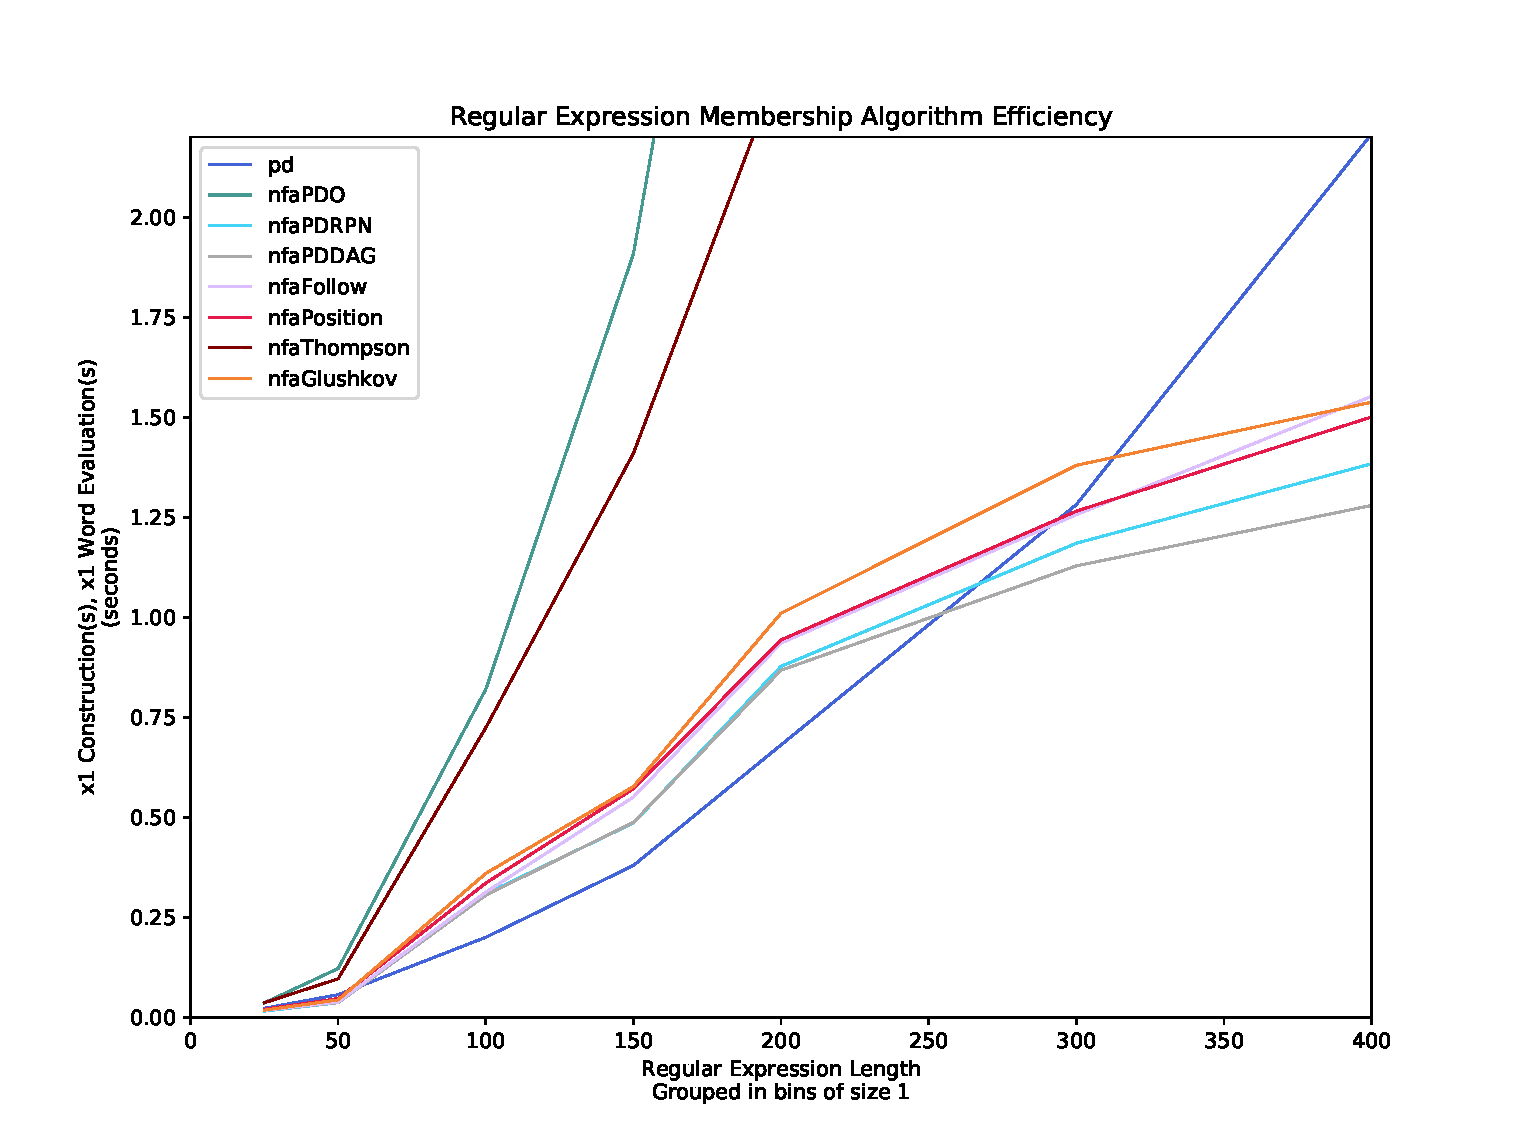
\includegraphics[width=0.75\linewidth]{fig/rand/1const1eval}
  \caption{Sum of construction time and one-word membership time for randomly generated regular expressions}
  \label{fig:rand/1const1eval}
\end{figure}

Figure \ref{fig:rand/1const1eval} combines Figures \ref{fig:rand/1construction} and \ref{fig:rand/1evaluation} to show how much time would be taken to construct the string into a Python class, and then evaluate membership of one word. The long length of input words makes determining word membership slow, so the construction cost is mostly negligible in comparison. The only significant difference from Figure \ref{fig:rand/1evaluation} is the nfaPDO construction makes this method the slowest, despite word membership on the partial derivative NFA being fast. The Thompson and nfaPDO methods are very slow, the partial derivative algorithm is competitively fast except at tree length 400, and then in increasing order: nfaPDDAG, nfaPDRPN, position, follow, and Glushkov.

\begin{figure}[H]
  \center
  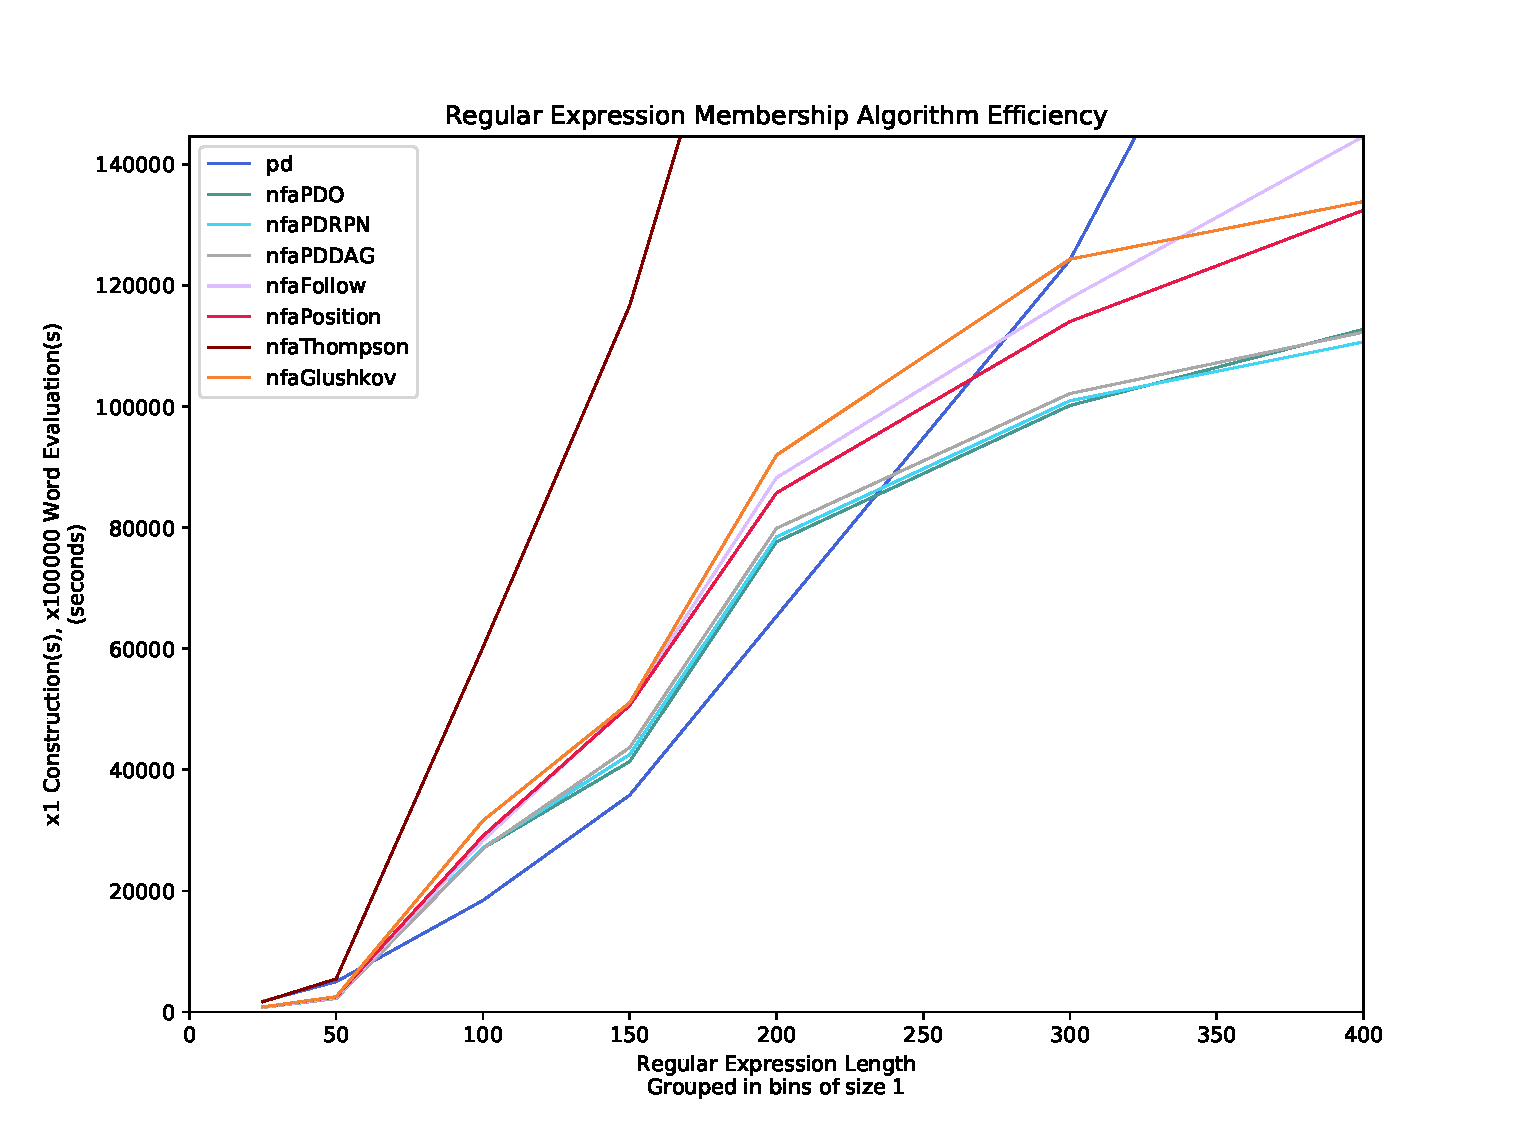
\includegraphics[width=0.75\linewidth]{fig/rand/1const10e6eval}
  \caption{Sum of construction time and 100,000 word membership time for randomly generated regular expressions}
  \label{fig:rand/1const10e6eval}
\end{figure}

There is little difference between Figure \ref{fig:rand/1const1eval} and Figure \ref{fig:rand/1const10e6eval}, only that the nfaPDO algorithm is once again competitive because the one-time construction cost is negligible in comparison to the membership cost.









